% xetex template
\documentclass[a4paper,11pt,onecolumn]{article}

\usepackage[top=20mm,bottom=20mm,left=20mm,right=20mm]{geometry}

\usepackage{xltxtra,fontspec,xunicode}

\usepackage{slantsc}
\usepackage[slantfont,boldfont]{xeCJK} % 允许斜体和粗体
\usepackage{ulem} % 斜线 波浪线 双下划线
\setCJKmainfont{Noto Sans CJK SC}   % 设置缺省中文字体
\setCJKmonofont{Noto Sans Mono CJK SC}   % 设置等宽字体
\setmainfont{Noto Serif}
\setsansfont{Noto Sans} % 英文无衬线字体
\setmonofont{Bitstream Vera Sans Mono}   % 英文等宽字体

% paragraph
\usepackage{indentfirst}
\setlength{\parindent}{2em}
\setlength{\parskip}{5pt}  % The space between paragraphs

% line
\usepackage{setspace}
\singlespacing
\frenchspacing % disable the additional space after periods

% for hyphenation if compound words that contain a dash
% \usepackage{hypenat}
% \tolerance=10000
% \hyphenpenalty=10000
\hbadness=5000
\emergencystretch=3em %\maxdimen

% for list
\usepackage[inline]{enumitem}
\setlist{leftmargin=2em}

% table
\usepackage{diagbox}
\usepackage{multirow}
\usepackage{longtable} % for table
\usepackage{booktabs} % for table
\usepackage[table]{xcolor}
\usepackage{array}

% code block
\usepackage{listings}
\usepackage{xcolor}

\lstdefinelanguage{bash}{
  keywords={type, function, return, in, for, while, until, do, done, if, else, elif, fi, then, case, break, continue, test},
  sensitive=true,
  comment=[l]{\#},
  morestring=[b]', % delimiter type: b -- backslash
  morestring=[b]",
  morestring=[b]`,
}

\lstnewenvironment{lstbash}
  {
    \lstset{
      language=bash,
      tabsize=4,
      showtabs=false,
      frame=shadowbox, % 把代码用带有阴影的框圈起来
      numbers=none,    % 左侧显示行号 往左靠,还可以为right,或none,即不加行号
      numbersep=0pt,   % 设置行号与代码的距离,默认是5pt
      numberstyle={\color[RGB]{0,192,192}\tiny}, % 设置行号的大小,大小有tiny,scriptsize,footnotesize,small,normalsize,large等
      stepnumber=1, % 若设置为2,则显示行号为1,3,5,即stepnumber为公差,默认stepnumber=1
      showspaces=false,
      showstringspaces=false, % 不显示代码字符串中间的空格标记
      flexiblecolumns=true,
      breaklines=true, % 对过长的代码自动换行
      breakautoindent=true,
      breakindent=2em,
      aboveskip=1em,   % space between code block and other block
      belowskip=0em,
      escapeinside={(*@}{@*)},
      framextopmargin=2pt,framexbottommargin=2pt,
      abovecaptionskip=0pt,belowcaptionskip=0pt,
      xleftmargin=1em,xrightmargin=1em, % 设定listing左右的空白
      texcl=false,  % 设定中文冲突,断行,列模式,数学环境输入,listing数字的样式
      mathescape=false,
      extendedchars=false,
      basicstyle=\ttfamily, % 这句设置代码的大小
      backgroundcolor=\color[RGB]{245,245,244},   %代码背景色
      rulesepcolor=\color{red!20!green!20!blue!20},%代码块边框为淡青色
      keywordstyle=\color{blue!90}\bfseries, %代码关键字的颜色为蓝色,粗体
      identifierstyle=\color{black},
      commentstyle=\color{purple}\ttfamily,
      stringstyle=\color{red}\ttfamily,
      %caption=\lstname,
      literate={\$}{{\textcolor{blue}{\$}}}1
    }
  }
{}

\lstset{
  alsolanguage=C,
  alsolanguage=C++,
  tabsize=4,
  showtabs=false,
  frame=shadowbox, % 把代码用带有阴影的框圈起来
  numbers=none,    % 左侧显示行号 往左靠,还可以为right,或none,即不加行号
  numbersep=0pt,   % 设置行号与代码的距离,默认是5pt
  numberstyle={\color[RGB]{0,192,192}\tiny}, % 设置行号的大小,大小有tiny,scriptsize,footnotesize,small,normalsize,large等
  stepnumber=1, % 若设置为2,则显示行号为1,3,5,即stepnumber为公差,默认stepnumber=1
  showspaces=false,
  showstringspaces=false, % 不显示代码字符串中间的空格标记
  stringstyle=\ttfamily,  % 代码字符串的特殊格式
  flexiblecolumns=true,
  breaklines=true, % 对过长的代码自动换行
  breakautoindent=true,
  breakindent=2em,
  aboveskip=1em,   % space between code block and other block
  belowskip=0em,
  escapeinside={(*@}{@*)},
  framextopmargin=2pt,framexbottommargin=2pt,
  abovecaptionskip=0pt,belowcaptionskip=0pt,
  xleftmargin=1em,xrightmargin=1em, % 设定listing左右的空白
  texcl=false,  % 设定中文冲突,断行,列模式,数学环境输入,listing数字的样式
  mathescape=false,
  extendedchars=false,
  basicstyle=\ttfamily, % 这句设置代码的大小
  backgroundcolor=\color[RGB]{245,245,244},   %代码背景色
  rulesepcolor=\color{red!20!green!20!blue!20},%代码块边框为淡青色
  keywordstyle=\color{blue!90}\bfseries, %代码关键字的颜色为蓝色,粗体
  identifierstyle=\color{black},
  commentstyle=\color{purple}\ttfamily,
  stringstyle=\color{red}\ttfamily,
  captionpos=b,
}

% Causes clash if hyperref parameters loaded before bookmark,
% because bookmark loads hyperref without any parameters
\usepackage[anchorcolor=blue,citecolor=green]{hyperref}
\usepackage{bookmark}
\usepackage{graphicx} % also for scalebox
\usepackage{caption}
\usepackage{subcaption} % subfigure
\usepackage{float}
\captionsetup{
  justification=raggedright, % centering
  singlelinecheck = false
}

\hypersetup{colorlinks=true,linkcolor=red,hypertexnames}

\begin{document}

\title{PDF 文档模板}
\author{Xin Xu}

\maketitle
\tableofcontents

\newpage

\section{一级标题}

\subsection{二级标题}

\subsubsection{三级标题 列表}
\noindent
Ordered lists
\begin{enumerate}
\def\labelenumi{\arabic{enumi}.}

\setlength{\itemsep}{5pt}
\setlength{\partopsep}{0pt}
\setlength{\topsep}{5pt}

\item
  berief mode : \begin{enumerate*}[label={\alph*).},font={\color{red}\bfseries}]
    \item bananas
    \item apples
    \item oranges and
    \item lemons.
  \end{enumerate*}
\item
  罗马数字
  \begin{enumerate}[label={(\roman*).}]
    \item
      罗马数字 1
    \item
      罗马数字 2
  \end{enumerate}
\item
  阿拉伯数字
  \begin{enumerate}[label={\arabic*.}]
    \item
      阿拉伯数字 1
    \item
      阿拉伯数字 2
  \end{enumerate}
\item
  列表包含多张图片

  \begin{figure}[hbtp]
    \centering
    \begin{subfigure}[b]{0.2\linewidth}
      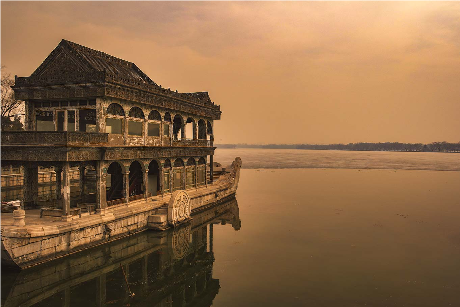
\includegraphics[width=\linewidth]{materials/boat.png}
      \caption{boat.}
    \end{subfigure}
    \begin{subfigure}[b]{0.2\linewidth}
      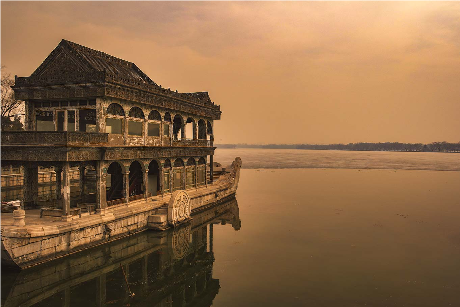
\includegraphics[width=\linewidth]{materials/boat.png}
      \caption{More boat.}
    \end{subfigure}
    \begin{subfigure}[b]{0.2\linewidth}
      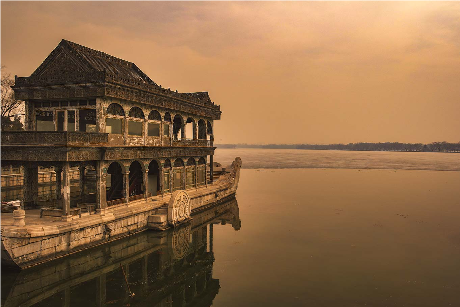
\includegraphics[width=\linewidth]{materials/boat.png}
      \caption{Tasty boat.}
    \end{subfigure}
    \begin{subfigure}[b]{0.5\linewidth}
      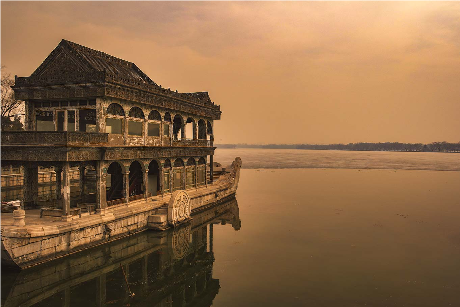
\includegraphics[width=\linewidth]{materials/boat.png}
      \caption{Too much boat.}
    \end{subfigure}
    \caption{The same boat. Multiple times.}
  \end{figure}
\end{enumerate}

Unordered lists
\begin{itemize}[label=$\ast$]
  \item One
    \begin{itemize}
      \item[--] Dash
      \item[$-$] Dash
      \item[$\ast$] Asterisk
    \end{itemize}
  \item Two
\end{itemize}
\subsubsection{三级标题 引用}
\begin{quote}
引用示例
  \begin{quote}
  引用引用示例
  \end{quote}
\end{quote}
\subsubsection{三级标题 段落}
% hang indent only for specific paragrah
% echo paragraph must set itself hange indent parameter
\hangafter 1 % hang indent after nth line in the current paragraph
\setlength{\hangindent}{2em} % size of hang indent
\noindent
这是悬挂缩进的演示。该段无首行缩进;从段落第二行开始悬挂缩进,悬挂缩进的距离为 2 个
m 的距离。正确的效果是该段落从第 2 行开始的每一行都会缩进 2em 的距离。

\parindent 1em
这是首行缩进的演示。该段落的首行会缩进 1em 的距离,其他行均不会缩进。正确的效果是
段落的首行缩进 1em 的距离。
\subsubsection{三级标题 字体、横线、删除线等}
\begin{itemize}
  \item 显示直立文本: $\backslash$textup\{文本\} \textup{Example}
  \item 意大利斜体: $\backslash$textit\{文本\} \textit{Example}
  \item slanted斜体: $\backslash$textsl\{文本\} \textsl{Example}
  \item 显示小体大写文本: $\backslash$textsc\{文本\} \textsc{Example}
  \item 中等权重: $\backslash$textmd\{文本\} \textmd{Example}
  \item 加粗命令: $\backslash$textbf\{文本\} \textbf{Example}
  \item 默认值: $\backslash$textnormal\{文本\} \textnormal{Example}
  \item 下划线:$\backslash$underline\{文字\} \underline{Example}
  \item 删除线:$\backslash$sout\{文字\} \sout{Example}
  \item 波浪线:$\backslash$uwave\{文字\} \uwave{Example}
  \item 斜删除线:$\backslash$xout\{文字\} \xout{Example}
  \item 双下划线:$\backslash$uuline\{文字\} \uuline{Example}
  \item 强调:$\backslash$emph\{文字\} \emph{Example}
  \item 字体背景色:$\backslash$colorbox{gray}{content} \colorbox{gray}{Example}
\end{itemize}
\subsubsection{三级标题 表格}
表格中单元格换行使用\colorbox{gray}{minipage + centerline 环境}进行长内容换行和居中,例如 Span two rows two columns 的换行。效果如 Table 1。
  \begin{lstlisting}
    \begin{minipage}{2cm}\centerline{居中}\end{minipage}
    \begin{minipage}{2cm}\centerline{Span two rows}\centerline{tow columns}\end{minipage}
  \end{lstlisting}

\begin{table}[H]\footnotesize
\centering
\caption{7x7 table a, span rows and columns}
\scalebox{1.5}{
\begin{tabular}{cc|c|l|c|r|l}
\cline{3-6}
 & & \multicolumn{4}{ c| }{Primes} \\ \cline{3-6}
 & & 3 & 4 & 5 & 6 \\ \cline{1-6}
\multicolumn{1}{ |c }{\multirow{2}{*}{Span two rows} } & \multicolumn{1}{ |c| }{2} & 3 & 4 & 5 & 6 & \\ \cline{2-6}
\multicolumn{1}{ |c }{}                                & \multicolumn{1}{ |c| }{2} & 3 & 4 & 5 & 6 & \\ \cline{1-6}
\multicolumn{2}{ |c }{\multirow{2}{*}{\begin{minipage}{2cm}\centerline{Span two rows}\centerline{tow columns}\end{minipage}} } & \multicolumn{1}{ |c| }{3} & 4 & 5 & 6 & min \\ \cline{3-6}
\multicolumn{2}{ |c }{}                                            & \multicolumn{1}{ |c| }{3} & 4 & 5 & 6 & max \\ \cline{1-6}
\end{tabular}
}
\label{table a:7x7 example}
\end{table}
表格单元格行高控制:
\begin{itemize}
  \item 通过\colorbox{gray}{$\backslash$$\backslash$ [3em]}这样的方式控制行高,会导致单元格内的内容无法垂直居中。
  \item 若是简单调整行距,则可以在插入表格前添加一行这样的命令:

    \begin{lstlisting}
    \renewcommand\arraystretch{1.5}
    \end{lstlisting}
  \item 精细调整使用表格线安装包,插入一个透明的表格线,通过控制表格线与内容的上下距离来控制行高

  specialrule 命令和示例:

    \begin{itemize}
      \item 第一个大括号控制表格线的粗细,若为0,则表格线透明
      \item 第二个大括号是表格线与上方内容的距离
      \item 第三个大括号是表格线与下方内容的距离
    \end{itemize}

    \begin{lstlisting}
    \usepackage{array}
    \usepackage{booktabs}
    \begin{tabular}
    \specialrule{0em}{1pt}{1pt}
    \end{tabular}
    \end{lstlisting}
\end{itemize}
\begin{table}[H]
\centering
\caption{3x3, 表格背景色 }
\rowcolors{2}{green}{pink}
\begin{tabular}[c]{llrm{5cm}}
odd  & \multicolumn{1}{>{\columncolor{red}}r}{\color{white}odd} & odd \\
even & even & p\{5cm\}控制列宽 \\
odd  & odd  & \begin{minipage}{0.2\textwidth}\centerline{控制行高并水平居中}\end{minipage} \\ [3em]
\rowcolor{white}
even & even & 单行设置白色 \\
\specialrule{.1em}{0pt}{10pt}
odd  & odd  & odd \\
\specialrule{.1em}{10pt}{0pt}
\end{tabular}
\end{table}

通过 \colorbox{gray}{m\{3cm\}<\{$\backslash$centering\}}的方式控制表格列内容的对齐方式。下面的 Table 3 显示具体的效果

\begin{table}[H]
\begin{tabular}{m{3cm}<{\centering}m{3cm}<{\raggedleft}l}
  \toprule
  odd  & odd  & odd \\ \cline{2-3}
  even & \multicolumn{2}{|c|}{ \multirow{2}{*}{\diagbox[dir=SW,width=16em,height=2em,trim=r]{A}{B}} } \\
  odd  & \multicolumn{2}{|c|}{ }                       \\ \cline{2-3}
  even & even & even \\
  \bottomrule
  \end{tabular}
  \caption{3x3, 对齐方式}
  \label{table b:3x3 example}
\end{table}

$\backslash$rowcolors 和 $\backslash$diagbox 以及 $\backslash$cline 等配合不是很好,容易出现颜色或者边框或者 diagbox 不符合预期的问题。效果如 Table 4。

\begin{table}[H]
  \rowcolors{1}{green}{pink}
  \caption{3x3, 边框颜色绘制出错}
  \begin{tabular}{llr}
  \toprule
  odd  & odd  & 跨行单元格导致颜色异常 \\ \cline{2-3}
  even & \multicolumn{2}{|c|}{ \multirow{2}{*}{\diagbox[dir=SW,width=14em,height=3em,trim=r]{A}{B}{C}} } \\ [1.5em]
  odd  & \multicolumn{2}{|c|}{ }                       \\ [1.5em] \cline{2-3}
  \hiderowcolors even & even & even \\
  \bottomrule
  \end{tabular}
  \label{table c:3x3 example}
\end{table}
\subsubsection{三级标题 代码块}
\begin{lstlisting}[language=C]
int main(int argc, char ** argv)
{
    printf("Hello world!\n");

    return 0;
}
\end{lstlisting}

\noindent
自定义语言 bash lstlisting 环境

\begin{lstbash}
#!/bin/bash

dest_dir="./copy_rename"
o_list=`find -name "*.o"`

i=0
for var in $o_list
do
  o_file=$var
  o_prefix=${var%/*.o}
  o_filename=${var##*/}
  echo "$o_prefix, $o_filename"

  if [ ! -d $dest_dir/$o_prefix ]; then
    mkdir -p $dest_dir/$o_prefix
  fi

  cp $o_file $dest_dir/$o_prefix/${o_filename}_$i

  i=$((i+1))
done
\end{lstbash}
\subsection{二级标题 正文}
\parindent 2em
正文 LaTex 示例
\end{document}
